\section{Техническое задание}
\subsection{Основание для разработки}

Основанием для разработки программы является задание на курсовую работу по дисциплине «Проектирование и архитектура программных систем» на тему «Разработка web-сайта «LeCourses-онлайн магазин курсов»»

\subsection{Цель и назначение разработки}

Основной задачей курсовой работы является разработка программы web-сайта онлайн магазина курсов.

Посредством создания конечной программы планируется устранить существующие проблемы в поиске курсов по программированию в интернете.

Задачами данной разработки являются:
\begin{itemize}
	\item создание интерфейса программы для пользователя;
	\item создание информационных разделов сайта;
	\item реализация формы для обратной связи;
	\item реализация формы для покупки курса;
	\item реализация добавления товара на сайт.
\end{itemize}

\subsection{Требования пользователя к интерфейсу программы}

Программа должна включать в себя:
\begin{itemize}
	\item навигацию по разделам;
	\item доступ для пользователя;
	\item покупку курса;
	\item авторизацию.
\end{itemize}

Композиция шаблона сайта представлена на рисунке ~\ref{плакат1:image}.

\begin{figure}[ht]
	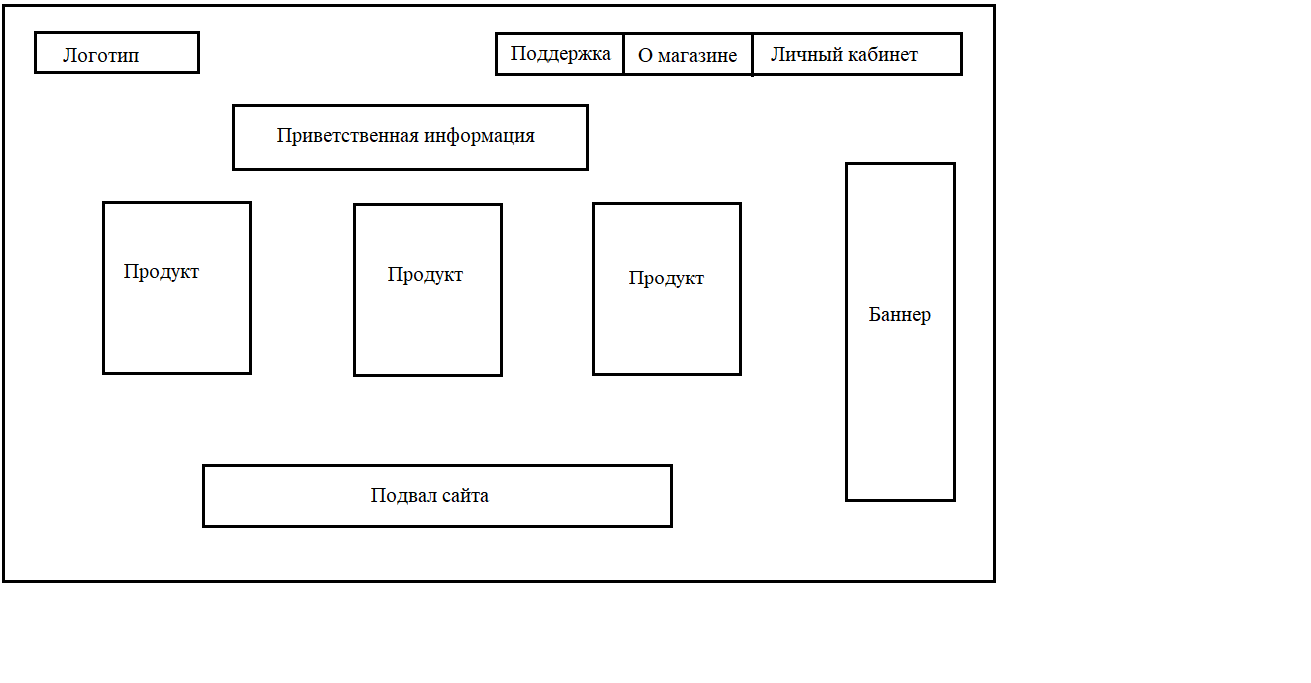
\includegraphics[width=1\linewidth]{плакат1}
	\caption{Композиция шаблона программы}
	\label{плакат1:image}
\end{figure}
%\vspace{-\figureaboveskip} % двойной отступ не нужен (можно использовать, если раздел заканчивается картинкой)

Диаграмма вариантов использования сайта представлена на рисунке ~\ref{прецедент:image}.

\begin{figure}[ht]
	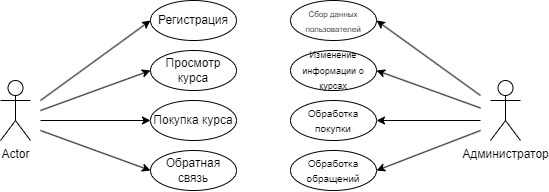
\includegraphics[width=1\linewidth]{прецедент}
	\caption{Композиция шаблона программы}
	\label{прецедент:image}
\end{figure}

\subsection{Моделирование вариантов использования}

Для разрабатываемой программы была реализована модель, которая обеспечивает наглядное представление вариантов использования сайта.

Она помогает в физической разработке и детальном анализе взаимосвязей объектов. При построении диаграммы вариантов использования применяется унифицированный язык визуального моделирования UML.

Диаграмма вариантов описывает функциональное назначение разрабатываемой системы. То есть это то, что система будет непосредственно делать в процессе своего функционирования. Она является исходным концептуальным представлением системы в процессе ее проектирования и разработки. Проектируемая система представляется в виде ряда прецедентов, предоставляемых системой актерам или сущностям, которые взаимодействуют с системой. Актером или действующим лицом является сущность, взаимодействующая с системой извне (например, человек, техническое устройство). Прецедент служит для описания набора действий, которые система предоставляет актеру.

На основании анализа предметной области в программе должны быть реализованы следующие прецеденты:
\begin{enumerate}
	\item просмотр информации о сайте;
	\item регистрация пользователя;
	\item реализация обратной связи;
	\item просмотр информации о курсе;
	\item покупка курса.
\end{enumerate}

\subsection{Требования к оформлению документации}

Разработка программной документации и программного изделия должна производиться согласно ГОСТ 19.102-77 и ГОСТ 34.601-90. Единая система программной документации.
